%% name       : Speptide.
%% description: Application to find amino acid substitution by spectra comparison.
%% author     : Dima Ischenko, Dima Alexeev
%% date       : 30/06/2016
%% make       : pdflatex speptide.tex


\documentclass{article}

% page settings
\usepackage[top=1.5in, bottom=1in, left=1in, right=1.5in]{geometry}
\usepackage{listings}
\usepackage{color}
\usepackage{enumerate}
\usepackage{indentfirst}
\usepackage{float}
\usepackage{graphicx}
\usepackage{enumitem}

% code style
\definecolor{dkgreen}{rgb}{0,0.6,0}
\definecolor{gray}{rgb}{0.5,0.5,0.5}
\definecolor{mauve}{rgb}{0.58,0,0.82}
\lstset{frame=tb,
  language=R,
  aboveskip=3mm,
  belowskip=3mm,
  showstringspaces=false,
  columns=flexible,
  basicstyle={\small\ttfamily},
  numbers=none,
  numberstyle=\tiny\color{gray},
  commentstyle=\color{dkgreen},
  stringstyle=\color{mauve},
  breaklines=true,
  breakatwhitespace=true
  tabsize=3
}


\title{\textbf{Speptide}. Application to find amino acids substitutions by spectra comparison.
       \\[3ex]
       \normalsize{version: 0.92.}}
\author{Dmitry Ischenko, Dmitry Alexeev, Ilya Altukhov}
\date{{\small\today}}

\begin{document}
\maketitle

\clearpage

\subsection{Intro}
\par
Spectide written at C/C++ language. The application allows you to determine the amino acid substitutions based on a comparison of the spectra. The basic idea of the spectrum as a vector, shifts of the peaks and the calculation of the angle between the vectors.

\subsection{Installation and usage}
\par
For installation just run:
\begin{lstlisting}
$ make
\end{lstlisting}
\par
in folder with project.\\
\par
To search for a substitutions you should have two sets of spectra. One -- experiment set of spectra and another -- database set of spectra (with SEQ= tag for each spectra). Both in Mascot Generic Format (.mgf).\\
\par
To create database spectra from \textbf{.mgf} and mascot result \textbf{.csv} file (it must contain columns with spectrum name ``pep\_scan\_title'' and peptide sequence ``pep\_seq'') -- use \textbf{mgfe.pl} script (utils/mgfe.pl):
\begin{lstlisting}
$ perl mgfe.pl mseq <mascot csv> <mgf> > <db mgf>
\end{lstlisting}
\par
Next. To run application:
\begin{lstlisting}
$ speptide <exp mgf> <db mgf> <config>
\end{lstlisting}
\par
Results in tab separated format:
\begin{lstlisting}
[exp spectrum id] [db spectrum id] [position] [exp ami] [db ami] [db seq] [cos(theta)]
\end{lstlisting}

\begin{lstlisting}
<exp spectrum id>  # experiment spectrum title
<db spectrum id>    # database spectrum title
<position>          # positions of substitution (if several space as delimiter)
<exp ami>           # aminoacid in experiment spectrum (substitution)
<db ami>            # aminoacid in database spectrum
<db seq>            # database spectrum sequence
<cos(theta)>        # cos(angle) between spectra
\end{lstlisting}


\clearpage
\subsection{Params}
\par

File with parameters (\textbf{.ini}) consists of several keys:
\begin{lstlisting}
# Default settings for algorithm

# Part for algorithm of idenitcal spectras
[ident]
ppm = 10;      # ppm accuracy for MS1 peak intersection
Da = 0.5;      # Da accuracy for MS2 peak intersection
N = 100;       # value for top (m / N) intensity peak selection
trans = b;     # algorightm for transfromation (a : sqrt, b : ln, c : none)
norm = y;      # normalize intensity
const = 0;     # add constant after normalization and transfromation 
cos01 = 0.47;  # value of threshold of cos(theta) (FDR <= 0.01)
cos05 = 0.3;   # value of threshold of cos(theta) (FDR <= 0.05)

# Part for algorithm for finding sap
[sap]
ppm = 10;      # ppm accuracy for MS1 peak intersection
Da = 0.5;      # Da accuracy for MS2 peak intersection
N = 3.2;       # value for top (N * S) intensity peak selection (S number of annotated peaks)
trans = b;     # algorightm for transfromation (a : sqrt, b : ln, c : none)
norm = y;      # normalize intensity
const = 0;     # add constant after normalization and transfromation
mcos = 0.3;    # value of threshold of cos(theta) for modification filtration
cos = 0;       # value of threshold of cos(theta) for printing
addions = n;   # additional ions (-H20, -NH3)
refdiv = 1;    # value for top (mz / N) intensity peak in reference (1 mean all)
fident = y;    # filter identical spectra from SP
fmod = y;      # filter modifications from SP

# Annotation params
[annot]
Da = 0.5       # Da accuracy for MS2 peak annotation
Ch = 2,3       # Add defalt charges (if didn't set in mgf)

\end{lstlisting}
\clearpage
\par
Training results:
\begin{figure}[H]
  \center{
  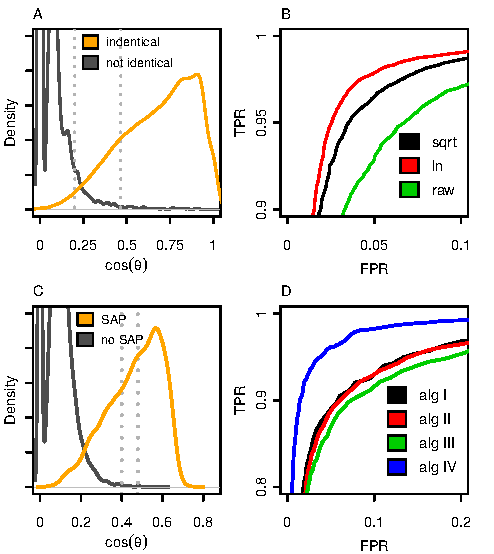
\includegraphics[scale=1.2]{./pics/Figure2.pdf}
  \caption{{\small 
\textbf{A}. Probability density of $\cos\Theta$ between the spectra, corresponding to similar and different peptide sequences ($\ln⁡ I$ transformation, top $\frac{m}{100}$ peaks). \textbf{B}. ROC curves for different methods of intensity transformation. \textbf{C}. Probability density of $\cos⁡\Theta$ between the spectra, corresponding to true SAP and random match (IV algorithm, $\ln⁡ I$ transformation, top $3.2 \dot S$ peaks). \textbf{D}. ROC curves for different methods of reference spectra transformation.
   }}
  }
 \end{figure} 


\clearpage
\subsection{Pipeline}
\begin{figure}[H]
  \center{
  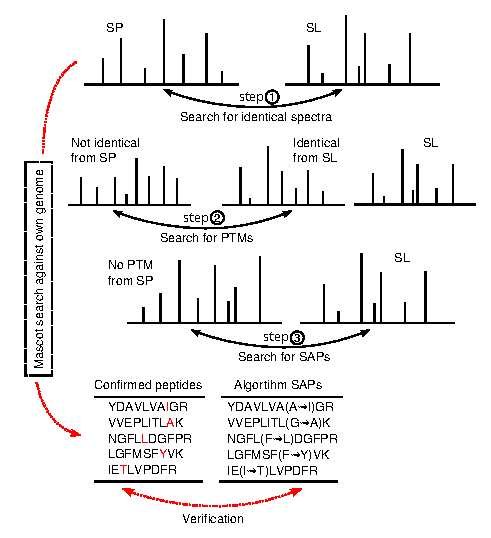
\includegraphics[scale=1.4]{./pics/Figure1.pdf}
  \caption{{\small Flowchart of algorithm for detecting the spectra with single amino acid substitution (steps 1-3) and additional verification procedure.}}
  }
\end{figure}

Application algorithm consists of several steps:\\
\begin{enumerate}
\item{Search for identical spectra in SP and SL. Filtration identical spectra from SP.}
\item{Search for PTM spectra in SP against identical form SL. Filtration PTM spectra from SP.}
\item{Search for SAPs.}
\end{enumerate}
\clearpage

\subsection{Example}
Graphical representation of the results of algorithm for several bacterial spectra datasets:
\begin{figure}[H]
  \center{
  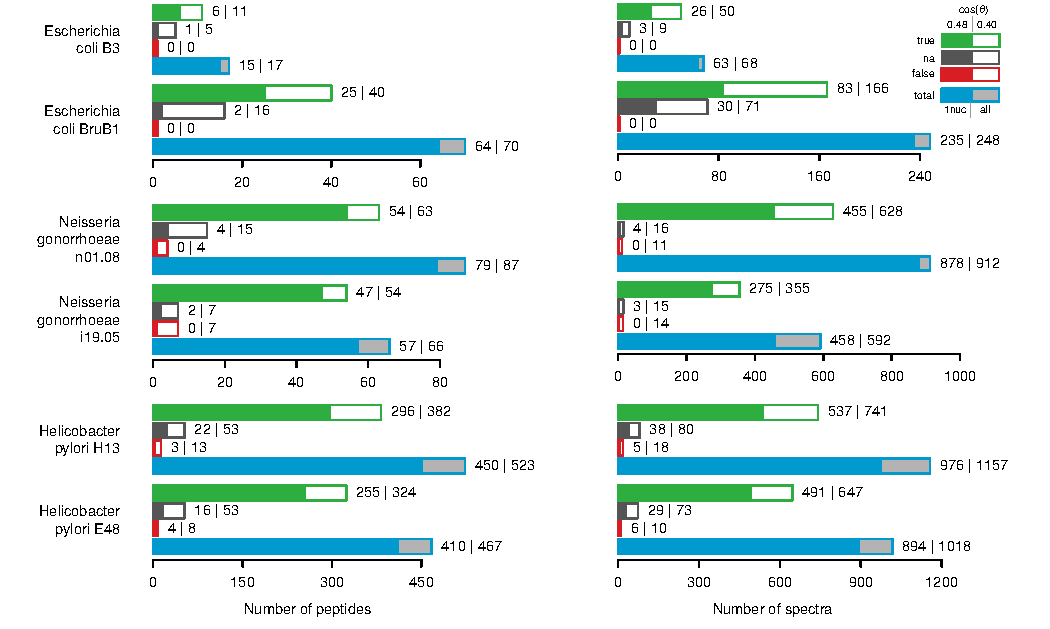
\includegraphics[scale=1]{./pics/Figure3.pdf}
  \caption{{\small Example of result of application for different bacterial datasets. }}
  }
 \end{figure} 

\subsection{Contribution}
\par
For comments and requests, send an email to:
\par
Dima Ischenko (ischenko.dmitry@gmail.com)

\end{document}
